\documentclass[pdf, unicode, 10pt, notheorems, handout]{beamer}

%\mode<handout> {
%    \usepackage{pgfpages}
%    \setbeameroption{show notes}
%    \pgfpagesuselayout{2 on 1}[a4paper, border shrink=5mm]
%    \setbeamercolor{note page}{bg=white}
%    \setbeamercolor{note title}{bg=gray!10}
%    \setbeamercolor{note date}{fg=gray!10}
%}

\usepackage[utf8]{inputenc}
\usepackage[T2A]{fontenc}
\usepackage[russian, english]{babel}
\usepackage{amsmath, amssymb, amsfonts}
\usepackage{graphics}
\usepackage{mathtools}
\usepackage{nicematrix}
\usepackage{multirow}
\usepackage{xcolor}
\usepackage{tikz}
\usetikzlibrary{tikzmark, calc, fit}

\usefonttheme[onlymath]{serif}
\usetheme[numbers, totalnumbers, compress, nologo]{Statmod}
\setbeamerfont{institute}{size=\normalsize}
\setbeamertemplate{navigation symbols}{}

\graphicspath{{../img}}

\input{letters_series_mathbb}
\setbeamercolor{bluetext_color}{fg=blue}
\newcommand{\bluetext}[1]{{\usebeamercolor[fg]{bluetext_color}#1}}
\setbeamercolor{redtext_color}{fg=red}
\newcommand{\redtext}[1]{{\usebeamercolor[fg]{redtext_color}#1}}

\makeatletter
\NewDocumentCommand{\overcolor}{mm}{\mathpalette\overundercolor@{\overline{#1}{#2}}}
\NewDocumentCommand{\undercolor}{mm}{\mathpalette\overundercolor@{\underline{#1}{#2}}}
\newcommand{\overundercolor@}[2]{\overundercolor@@#1#2}
\newcommand{\overundercolor@@}[4]{%
  % #1 = math style
  % #2 = command
  % #3 = math material
  % #4 = color
  \sbox\z@{$\m@th#1#3$}%
  \mathcolor{#4}{#2{\usebox\z@}}%
}
\makeatother

\newcommand{\iu}{\mathbf{i}}
\newcommand{\Tp}{\mathrm{T}}
\newcommand{\Hp}{\mathrm{H}}
\newcommand{\rank}{\operatorname{rank}}

\newtheorem{theorem}{Теорема}
\newtheorem{statement}{Утверждение}
\newtheorem{definition}{Определение}
\newtheorem{remark}{Замечание}

\title{Тензорный анализ сингулярного спектра}

\author{Хромов Никита Андреевич, гр.24.M22-мм}

\institute[Санкт-Петербургский Государственный Университет]{
  Санкт-Петербургский государственный университет\\
  Математическое моделирование, программирование и \\искусственный интеллект\\
  Статистическое моделирование\\
  \vspace{0.7cm}
Научный руководитель:  д.ф.-м.н. Голяндина Н.Э.}
%   \\Рецензент: к.ф.-м.н. Усевич К.Д.}

\date{Санкт-Петербург,\\ \number\year}

\begin{document}

\begin{frame}[plain, noframenumbering]
  \titlepage
\end{frame}

\section{Введение}\label{sec:intro}
\begin{frame}{Введение}
  $\tX^{(m)} = \left(x_1^{(m)}, x_2^{(m)}, \ldots,
  x_N^{(m)}\right)^{\rmT}$, $x_i \in \bbC$ ---
  временной ряд\\
  $\tX = \left(\tX^{(1)} : \tX^{(2)} : \ldots : \tX^{(M)}\right)$ ---
  $M$-канальный временной ряд\\ \vspace{0.2cm}
  $\tX = \tT + \tP + \tE$ \\
  $\tT$ --- медленно меняющаяся составляющая (тренд)\\
  $\tP$ --- периодическая составляющая (сезонность)\\
  $\tE$ --- случайная составляющая (шум)\\
  \vspace{0.2cm}

  \bluetext{Возможные задачи:}
  \begin{itemize}
    \item Выделение сигнала из ряда: нахождение $\tS = \tT + \tP$
    \item Разделение сигнала: нахождение составляющих $\tT$ и $\tP$
    \item Оценка параметров сигнала: определение периода и скорости
      изменения компонент сигнала
  \end{itemize}
  \smallskip

  Возможный метод решения: Singular Spectrum Analysis (\bluetext{SSA})

  %   [Broomhead, King (1986a)], [Golyandina, Nekrutkin, Zhigljavsky (2001)],\\
  %   и его многомерное расширение Multivariate SSA (\bluetext{MSSA})

  %   [Broomhead, King (1986b)]

  \smallskip

  \redtext{Цель:} сравнение и исследование свойств тензорных
  расширений методов SSA и MSSA с точки зрения точности выделения
  сигнала, разделения компонент и оценки параметров.
\end{frame}

\section{SSA}

\begin{frame}{Алгоиртм SSA}
  $\tX = \sum_{m=1}^{M}\tS_m + \tE$ --- временной ряд (один
  канал),\\ \vspace{0.1cm}
  $\tS \stackrel{\mathrm{def}}{=}\sum_{m=1}^{M}\tS_m$ ---
  сигнал.\\ \vspace{0.2cm}

  \bluetext{Параметры:} $L < N$ --- длина окна, $K
  \stackrel{\mathrm{def}}{=} N - L + 1$,\\
  $R$ --- число элементов разложения, относимых к сигналу,\\
  $\gI_1,\ldots, \gI_J \subseteq \{1, 2, \ldots, R\}$, $\gI_i \cap
  \gI_j = \varnothing$ --- наборы индексов,
  относимых к компонентам сигнала.
  \vspace{0.1cm}

  \bluetext{Алгоритм SSA для разделения компонент сигнала}
  \begin{enumerate}
    \item \bluetext{Вложение}
      $\tX \overset{L}{\longmapsto} \calT_L(\tX) = \bfX\in \bbC^{L\times K}$ ---
      траекторная матрица,

    \item \bluetext{Разложение} $\operatorname{SVD}(\bfX) =
      \sum_{i=1}^{\rank(\bfX)} \sqrt{\lambda}_{i}
      U_i V_i^{\Hp}
      $
    \item \bluetext{Группировка} $\widetilde{\bfS}_j = \sum_{\color{red} i\in
      \gI_j}\sqrt{\lambda}_{i} U_i V_i^{\Hp}, \quad R \leqslant \rank(\bfX)
      $
    \item \bluetext{Восстановление} усреднение $\widetilde{\bfS}_j$
      вдоль антидиагоналей $l+k=\operatorname{const}$
  \end{enumerate}
  \vspace{0.1cm}

  \bluetext{Результат алгоритма} $\widetilde{\tS}_j$ --- оценки
  компонент $\tS_j$
\end{frame}

\begin{frame}{Траекторная матрица ряда}
  $\tX = (x_1,\, x_2,\, \dots,\, x_N)$, $L < N$, $K = N - L + 1$
  \vspace{0.4cm}\\
  \begin{definition}
    \[
      \bfX = \calT^{(L)}(\tX) =
      \begin{pmatrix}
        x_1                     & \tikzmarknode{A12}{x_2} &
        \tikzmarknode{A13}{x_3} & \ldots & x_K     \\
        \tikzmarknode{A21}{x_2} & x_3                     & x_4
        & \ldots & x_{K+1} \\
        \tikzmarknode{A31}{x_3} & x_4                     & x_5
        & \ldots & x_{K+2} \\
        \vdots                  & \vdots                  & \vdots
        & \ddots & \vdots  \\
        x_L                     & x_{L+1}                 & x_{L+2}
        & \ldots & x_N
      \end{pmatrix}
    \]
    \begin{tikzpicture}[remember picture,overlay]
      \draw[red] let \p1=($(A12)-(A21)$),\n1={atan2(\y1,\x1)} in
      node[rotate fit=\n1,fit=(A12) (A21),draw,rounded
      corners,inner sep=2pt]{};
      \draw[blue] let \p1=($(A13)-(A31)$),\n1={atan2(\y1,\x1)+2} in
      node[rotate fit=\n1,fit=(A13) (A31),draw,rounded
      corners,inner sep=2pt]{};
    \end{tikzpicture}
  \end{definition}
  \bigskip

  Шаг восстановления: $\widetilde{\tS} =
  \calT_L^{-1}\left(\Pi_{\calH}\left(\bfS_j\right)\right)$,\\
  $\Pi_{\calH}$ --- проектор на пространство ганкелевых матриц.
\end{frame}

\begin{frame}{SSA-Ранг Ряда}
  \begin{definition}
    Ряд $\tX$ имеет SSA-ранг $\rank(\tX)=r < N/2$, если ранг его $L$-траекторной
    матрицы равен $r$ для любой длины окна $L$ такой, что $r
    \leqslant \min(L, K)$.\\
    Если такое число $r$ существует, тогда ряд $\tX$ называется рядом
    конечного ранга.
  \end{definition}
  \vspace{0.5cm}
  Если сигнал $\tS$ является рядом конечного ранга, то в общем случае
  рекомендуется использовать $\rank(\tS)$ в качестве параметра $R$ в
  алгоритме SSA.
  \vspace{0.4cm}\\
  Примеры SSA-рангов
  \begin{itemize}
    \item ранг $\tS$ при $s_n = A \exp(\alpha n)$, $\alpha
      \in\bbC$, равен 1
    \item ранг $\tS$ при $s_n = A\sin(2\pi \omega n + \varphi)$,
      $0 < \omega < 1/2$, равен 2
  \end{itemize}
\end{frame}

\begin{frame}{Модель Сигнала}
  Ряд $\tS = (s_1,\, s_2,\, \ldots, s_N)$ считается сигналом, если
  траекторная матрица $\bfS = \calT^{(L)}(\tS)$ имеет неполный ранг
  ($\implies$ ряд имеет конечный $L$-ранг:
  $\rank_L(\tS)=r$)

  \bigskip

  Любой сигнал конечного ранга $\tS$ представим в форме конечной суммы:
  \[
    s_n = \sum_{j} p_j(n) \exp(\alpha_j n + \mathrm{i}2\pi
    \omega_j n),
  \]
  где $p_j(n)$ --- некоторый многочлен от $n$

  \bigskip

  Вещественный случай:
  \[
    s_n = \sum_{j} p_j(n) \exp(\alpha_j n)\sin(2\pi
    \omega_j n + \varphi_j),
  \]

  \medskip

  ESPRIT --- метод оценки степеней $\alpha_j$ и частот $\omega_j$,
  основанный на подпространстве сигнала

  %   [Roy et al. (1986)]
\end{frame}

\begin{frame}{Алгоритм ESPRIT}
  Входные данные: ряд $\tX$, длина окна $L$, число компонент сигнала $R$

  \bluetext{Алгоритм ESPRIT}
  \begin{enumerate}
    \item \bluetext{Вложение} $\bfX = \calT^{(L)}(\tX)$
    \item \bluetext{Разложение} $\displaystyle\bfX =
      \sum_{i=1}^{\rank\bfX}
      \sqrt{\lambda_i} U_i V_i^{\Hp}$,
      $\bfU_R = \left[U_1: U_2: \ldots: U_R\right]$
    \item \bluetext{Оценивание} Вычисление собственных чисел $z_j$ матрицы
      $\underline{\bfU}_R^{-}\overline{\bfU}_R$ \\ \smallskip
      Из равенства $z_j = \exp(\alpha_j + \mathrm{i}2\pi\omega_j)$ находятся
      параметры $\alpha_j$ и $\omega_j$.
  \end{enumerate}

  \bigskip

  Методы SSA, ESPRIT и их модификации называются методами,
  основанными на подпространстве сигнала.
\end{frame}

\section{Multi-Channel SSA}
\begin{frame}{MSSA: SSA для многоканальных рядов}
  %   [Broomhead, King (1986)]\\ \smallskip
  $\tX = \left(\tX^{(1)},\, \tX^{(2)}, \, \ldots,\,
  \tX^{(M)}\right)$ --- многоканальный ряд,
  $\tX^{(m)} = \left(x_1^{(m)}, \, x_2^{(m)},\,\ldots,\,
  x_N^{(m)}\right)$ --- каналы
  \vspace{0.4cm}

  Единственные отличия от алгоритма SSA --- шаг Вложения:
  \[
    \bfX = \calT_{\textrm{MSSA}}^{(L)}(\tX) = \left[\bfX^{(1)} :
    \bfX^{(2)}: \ldots : \bfX^{(M)}\right],\quad
    \bfX^{(m)} = \calT^{(L)}(\tX^{(m)}),
  \]
  и соответствующее изменение шага Восстановления.
  \vspace{0.4cm}

  Когда MSSA оказывается точнее, чем применение SSA к каждому каналу:
  \begin{itemize}
    \item Интерес представляют несколько каналов с ``похожей'' структурой
    \item Интерес представляет один рад, и имеются ``поддерживающие''
      каналы с меньшим уровнем шума
  \end{itemize}
\end{frame}

\section{Известные результаты. Тензоризация SSA}
\begin{frame}{Переход к тензорам}
  \begin{table}
    \hspace*{-0.9cm}
    \begin{tabular}{rlllll}
      \bluetext{Basic SSA:} & Ряд $\tX$ & $\mapsto$ & Матрица
      $\mathbf{X}$ & $\mapsto$ & $\operatorname{SVD}(\mathbf{X})$ \\
      \bluetext{Tensor SSA:} & Ряд $\tX$ & $\mapsto$ & Тензор
      $\calX $ & $\mapsto$ & \hspace*{-0.18cm}
      $\underbrace{\operatorname{TD}}_{\mathclap{\text{~~~Тензорное
      Разложение}}}(\calX)$
    \end{tabular}
  \end{table}
  \vspace{0.4cm}

  Тензорные разложения, обобщающие SVD:
  \begin{itemize}
    \item Разложение Таккера (в частности \bluetext{Higher-Order SVD (HOSVD)})
    \item Каноническое Полиадическое Разложение (CPD)
    \item T-SVD
    \item $(L_r, L_r, 1)$-Разложение
  \end{itemize}
\end{frame}

\begin{frame}{Вложение одноканального ряда в Тензор}
  Предложено в работе [Papy et al. (2005)]\\ \smallskip
  $\tX = (x_1,\, x_2,\, \ldots,\, x_N)$, $L, K < N - 1$, $M = N - L -
  K + 2 > 1$\\ \smallskip
  $\tX \mapsto \calT_{\mathrm{T-SSA}}^{(L, K)}(\tX) = \calX \in
  \bbC^{L\times K \times M}$:

  \begin{figure}[!ht]
    \centering
    
\includegraphics[width=0.75\textwidth]{tens-injection-wide.pdf}
  \end{figure}
\end{frame}

\begin{frame}{Вложение многоканального ряда в Тензор}
  Предложено в работе [Papy et al. (2005)]\\ \smallskip
  $\tX = \left(\tX^{(1)},\, \tX^{(2)},\, \ldots,\,
  \tX^{(M)}\right)$, $\tX^{(m)} = (x_1^{(m)},\, x_2^{(m)},\,
  \ldots,\, x_N^{(m)})$, $L < N$\\ \smallskip
  $\tX \mapsto \calT_{\mathrm{T-MSSA}}^{(L)}(\tX)
  = \calX \in \bbC^{L \times K \times M}$, $K = N - L + 1$

  \bigskip

  \begin{figure}[!ht]
    \centering
    
\includegraphics[width=\textwidth]{mssa_injection_new.pdf}
  \end{figure}
\end{frame}

\begin{frame}{Некоторые тензорные разложения}
  В отличие от матричного случая, существует несколько различных
  определений тензорных рангов и соответствующих им обобщений SVD.

  \begin{definition}[Ранг тензора]
    Тензор $\calA$ имеет ранг 1, если существуют векторы $B$, $C$ и
    $D$ такие, что
    $\calA=B \circ C \circ D$, где $\circ$ обозначает тензорное
    произведение.\\ \medskip

    Тензор $\calA$ имеет ранг $R$, если его можно представить в виде суммы
    $R$ одноранговых тензоров: $\calA = \sum_{i=1}^{R} \calB_i$,
    $\rank(\calB_i)=1$, и такое $R$ минимально.
  \end{definition}

  \medskip

  \bluetext{Каноническое Полиадическое Разложение (CPD)} --- представление
  тензора в виде суммы $R$ одноранговых тензоров.

  \smallskip

  \begin{itemize}
      % \item Considered for signal extraction in [Kouchaki, Sanei (2013)]
    \item Компоненты разложения не ортогональны
    \item Необходимо знать параметр $R$ до разложения
    \item Нет связи между SSA-рангом и рангом траекторного тензора
  \end{itemize}
\end{frame}

\begin{frame}{Некоторые тензорные разложения}
  \begin{definition}
    \bluetext{$n$-векторами} тензора $\calA$ называются векторы,
    получаемые из $\calA$ варьированием индекса $n$-го направления
    при фиксированных остальных (аналог строк и столбцов матрицы).\\ \smallskip

    \bluetext{$n$-развёрткой} тензора $\calA$ называется матрица
    $[\bfA_n]$, некоторым образом составленная из всех $n$-векторов
    тензора $\calA$.\\ \smallskip

    \bluetext{$n$-рангом} тензора $\calA$, обозначаемым $R_n =
    \rank_n(\calA)$, называется ранг $n$-развёртки этого тензора.
  \end{definition}

  \medskip

  \bluetext{HOSVD}: $\calA = \sum_{l=1}^{R_1}\,
  \sum_{k=1}^{R_2}\, \sum_{m=1}^{R_3}\, \calZ_{lkm} U_l^{(1)} \circ
  U_k^{(2)} \circ U_m^{(3)}$
  \begin{itemize}
      % \item Considered for signal parameter estimation in [Papy et
      %   al. (2005)], [Papy et al. (2009)]
    \item Компоненты разложения ортогональны
    \item Не требует заранее знать $n$-ранги тензора
    \item Была доказана связь между SSA-рангом
      сигналов и $n$-рангами их траекторных тензоров [Хромов (2024)]
  \end{itemize}
\end{frame}

\section{Известные результаты. HOSVD}
% \begin{frame}{Описание HOSVD}
%   $\calA \in \bbC^{I_1 \times I_2 \times I_3}$, тогда
%   $\operatorname{HOSVD}(\calA)$:
%   % Пусть имеется тензор $\calA\in \mathbb{C}^{I_1\times I_2
%   % \times \ldots \times I_M}$, тогда HOSVD $\calA$:

%   \begin{equation*}
%     \calA  = \sum_{i_1=1}^{I_1} \sum_{i_2=1}^{I_2} \sum_{i_3=1}^{I_3}
%     \calZ_{i_1 i_2 i_3}
%     U_{i_1}^{(1)} \circ U_{i_2}^{(2)} \circ U_{i_3}^{(3)},
%     % \calA=\sum_{i_1=1}^{I_1} \sum_{i_2=1}^{I_2}\ldots
%     % \sum_{i_M=1}^{I_M} \calZ_{i_1,i_2,\ldots,i_M}
%     % U^{(1)}_{i_1} \circ U^{(2)}_{i_2} \circ \ldots\circ U^{(M)}_{i_M},
%   \end{equation*}
%   где
%   \begin{itemize}
%     \item $\mathbf{U}^{(n)}=\left[U^{(n)}_{1}, \ldots,
%       U^{(n)}_{I_n}\right]$  --- унитарные матрицы;
%       \smallskip
%     \item Тензор $\calZ\in\mathbb{C}^{I_1\times I_2 \times
%       I_3}$ удовлетворяет свойствам:
%       \begin{enumerate}
%         \item полная ортогональность:
%           \[
%             \langle\mathcal Z_{i_n=\alpha},\mathcal
%             Z_{i_n=\beta}\rangle=0 \qquad \alpha\ne\beta,
%           \]
%         \item упорядоченность:
%           \begin{equation*}
%             \|\mathcal Z_{i_n=1}\|\geqslant\|\mathcal Z_{i_n=2}\|
%             \geqslant \ldots \geqslant\|\mathcal Z_{i_n=I_n}\|.
%           \end{equation*}
%       \end{enumerate}
%   \end{itemize}
% \end{frame}

% \begin{frame}{Свойства HOSVD}
%   Все свойства представлены в работе [De Lathauwer et al. (2000)].
%   \begin{itemize}
%     \item HOSVD --- единственное 3-ортогональное разложение.
%       \vspace{0.3cm}
%     \item Если $I_n=1$ для некоторого $n$ (тензор --- матрица), то
%       HOSVD совпадает с SVD.
%       \vspace{0.3cm}
%     \item Если в HOSVD тензора $\calA$ $r_n$ --- наибольший индекс
%       такой, что $\|\calZ_{i_n=r_n}\|>0$,
%       то $r_n=\rank_n(\calA)$.
%       \vspace{0.3cm}
%     \item
%   \end{itemize}
%   \vspace*{-0.7cm}
%   \begin{gather*}
%     \|\calA\|^2=\sum_{i=1}^{R_1}\left( \sigma_i^{(1)}
%     \right)^2=\sum_{i=1}^{R_2}\left( \sigma_i^{(2)} \right)^2
%     =\sum_{i=1}^{R_3}\left( \sigma_i^{(3)} \right)^2=
%     \|\calZ\|^2\\
%     \sigma_{i}^{(n)}=\|\calZ_{{i_n}=i}\|, \qquad
%     R_n=\rank_n(\calA).
%   \end{gather*}
%   % \end{itemize}
% \end{frame}

% \begin{frame}{Свойства HOSVD}
%   \begin{itemize}
%     \item $n$-векторы $\calA$ содержат наибольший вклад в направлении
%       $U^{(n)}_1$,
%       величина этого вклада равна $\sigma^{(n)^2}_1$.
%       Следующий по величине вклад по измерению $n$ достигается в
%       направлении $U^{(n)}_2$, перпендикулярном $U^{(n)}_1$, с
%       величиной $\sigma^{(n)^2}_2$, и т.д.
%       \vspace{0.4cm}
%     \item Определим тензор $\widehat{\calA}$ отсечением
%       наименьших сингулярных значений $\sigma_{I_{n}'+1}^{(n)},
%       \sigma_{I_{n}'+2}^{(n)},\ldots, \sigma_{R_n}^{(n)}$, тогда
%       \begin{equation*}
%         \|\calA-\widehat{\calA}\|^2\leqslant
%         \sum_{i_1=I_{1}'+1}^{R_1}\left( \sigma_{i_1}^{(1)}\right)^2 +
%         \sum_{i_2=I_{2}'+2}^{R_2}\left( \sigma_{i_2}^{(2)}\right)^2 +
%         \sum_{i_3=I_{3}'+1}^{R_3}\left( \sigma_{i_3}^{(3)}\right)^2.
%       \end{equation*}
%   \end{itemize}
% \end{frame}

\begin{frame}{Неоптимальность усечения}
  \vspace*{-0.7cm}
  \begin{align*}
    \operatorname{SVD}(\bfX) &= \sum_{i=1}^{\operatorname{rank}(\bfX)}
    \sqrt{\lambda_j} U_i V_i^{\Hp}\\
    \operatorname{HOSVD}(\calX) &=
    \sum_{i_1=1}^{\rank_1(\calX)}\,
    \sum_{i_2=1}^{\rank_2(\calX)}\,
    \sum_{i_3=1}^{\rank_3(\calX)}\,
    \calZ_{i_1 i_2 i_3} U_{i_1}^{(1)} \circ U_{i_2}^{(2)} \circ U_{i_3}^{(3)}
  \end{align*}

  \vspace*{-0.2cm}

  \begin{itemize}
    \item $\displaystyle \widetilde{\bfX} =
      \sum_{i=1}^{R}\ldots \Rightarrow
      \left\| \bfX - \widetilde{\bfX} \right\|_{\rmF} =
      \min_{\rank(\widehat{\bfX}) \leqslant R}\left\|
      \bfX - \widehat{\bfX}\right\|_\rmF$
    \item $\displaystyle \widetilde{\calX}=
      \sum_{i_1=1}^{R_1}\,
      \sum_{i_2=1}^{R_2}\,
      \sum_{i_3=1}^{R_3}\,
      \ldots \Rightarrow
      \left\| \calX - \widetilde{\calX} \right\|_{\rmF} \geqslant
      \min_{\operatorname{rank}_{m}(\widehat{\calX}) \leqslant R_m}\left\|
      \calX - \widehat{\calX}\right\|_\rmF$
  \end{itemize}
  \vspace{0.2cm}

  \bluetext{Усечение SVD оптимально, а усечение HOSVD -- нет}

  \vspace{0.2cm}

  \bluetext{Higher-Order Orthogonal Iteration (HOOI):}

  \vspace*{-0.1cm}

  \[
    \widetilde{\calX} =
    \operatorname{HOSVD}\left(\arg\min_{\calY}\left\|\calX -
    \calY \right\|_{\rmF} \right),
    \quad \rank_n\left(\calY\right) \leqslant R_n
  \]

\end{frame}

\begin{frame}{Вычисление HOSVD}
  Вычисление HOSVD тензора $\calA$ сводится к следующим шагам: \medskip

  \begin{enumerate}
    \item Применение SVD к $n$-развёрткам $[\bfA_n]$ для нахождения
      матриц левых сингулярных векторов $\bfU_n$ \smallskip
    \item Нахождение <<ядерного>> тензора:
      \[
        \calZ = \calA \times_1 \bfU_1^{\Hp} \times_2 \bfU_2^{\Hp}
        \times_3 \bfU_3^{\Hp}
      \]
  \end{enumerate} \medskip

  $\times_n$ обозначает умножение тензора на матрицу в направлении
  $n$\\
  В матричном случае для $\bfB \in \bbC^{I_b\times J_b}$, $\bfC \in
  \bbC^{I_c\times I_b}$, $\bfD \in \bbC^{I_d\times J_b}$:
  \[
    \bfB \times_1 \bfC = \bfC \bfB \in \bbC^{I_c \times J_b}
  \]
  \[
    \bfB \times_2 \bfD = \bfB \bfD^{\Tp} \in \bbC^{I_b \times J_d}
  \]
\end{frame}

\begin{frame}{Разложения Таккера}
  \begin{itemize}
    \item Разложением Таккера тензора $\calA$ называется его
      представление в виде
      \[
        \calA = \calZ \times_1 \bfU_1 \times_2 \bfU_2 \times_3 \bfU_3,
      \]\smallskip

    \item HOSVD --- частный случай разложения Таккера, в котором
      \begin{enumerate}
        \item Матрицы $\bfU_n$ унитарные
        \item Слои каждого направления $\calZ$ ортогональны между собой
      \end{enumerate}\smallskip

    \item Пусть $\calA = \calZ \times_1 \bfU_1 \times_2 \bfU_2
      \times_3 \bfU_3$ --- произвольное разложение Таккера, где $\bfU_n$
      --- унитарные матрицы. Если $\widetilde{\bfU}_n = \bfU_n \bfQ_n$, где
      $\bfQ_n$ --- матрицы поворота, то
      \[
        \calA = \widetilde{\calZ} \times_1 \widetilde{\bfU}_1
        \times_2 \widetilde{\bfU}_2 \times_3 \widetilde{\bfU}_3
      \]
      также является разложением Таккера с
      \[
        \widetilde{\calZ} = \calA \times_1 \widetilde{\bfU}_1^{\Hp} \times_2
        \widetilde{\bfU}_2^{\Hp} \times_3 \widetilde{\bfU}_3^{\Hp}
      \]

  \end{itemize}
\end{frame}

\section{Известные результаты. Алгоритмы T-SSA}
\begin{frame}{T-SSA, T-MSSA и T-ESPRIT с использованием HOSVD}
  \bluetext{Входные данные} временной ряд $\tX$,
  длина окна: $(L, K)$ для одноканальных рядов или $L$ для многоканальных,
  количество компонент сигнала для каждого направления
  $(R_1,\, R_2,\, R_3)$, номер направления оценки для T-ESPRIT $d$.
  \vspace{0.2cm}\\
  \begin{enumerate}
    \item \bluetext{Вложение}.
      \begin{tabular}{r|l}
        Одноканальный & $\tX \mapsto\calT_{\mathrm{T-SSA}}^{(I,
        L)}(\tX) = \calX$ \\ \hline
        Многоканальный &
        $\tX \mapsto \calT_{\mathrm{T-MSSA}}^{(L)}(\tX) = \calX$
      \end{tabular}
      \vspace{0.15cm}

    \item \bluetext{Разложение и Приближение}. Используя $(R_1,\,
      R_2,\, R_3)$\\\smallskip
      $\calX \mapsto \operatorname{Dec} (\calX) = \widetilde{\calS}$,
      где $\operatorname{Dec}(\calX) =
      \operatorname{Trunc}_{R_1,R_2,R_3}(\operatorname{Tucker}(\calX))$ или
      $\operatorname{HOOI}_{R_1,R_2,R_3}(\calX)$
      \vspace{0.15cm}

    \item \bluetext{Восстановление или Оценивание}. \\
      \begin{itemize}
        \item \bluetext{Восстановление}.
          $\tS = \calT^{-1}
          \left(\Pi_{\calH_{\mathrm{T}}} (\widetilde{\calS})\right)$,
          $\Pi_{\calH_{\mathrm{T}}}$ --- проектор на пространство
          Ганкелевых тензоров
        \item \bluetext{Оценивание}. Вычисление собственных чисел
          $z_j$ матрицы $\underline{\bfU}^{-}\overline{\bfU}$, где
          $\bfU = \bfU_d = \left[U_1^{(d)}:U_2^{(d)}:\ldots
          :U_{R_d}^{(d)}\right]$.
          Из равенства $z_j = \exp(\alpha_j + \mathrm{i}2\pi\omega_j)$
          находятся степени $\alpha_j$ и частоты $\omega_j$.
      \end{itemize}
  \end{enumerate}
\end{frame}

\section{Постановка задачи}
\begin{frame}{Цели и необходимые результаты}
  \begin{enumerate}
    \item Разновидности задач
      \begin{itemize}
        \item Выделение сигнала -- разделение компонент -- оценка параметров
        \item Одноканальный ряд -- многоканальный ряд
        \item Вещественный ряд -- комплексный ряд
      \end{itemize}\medskip
    \item Подбор параметров метода
      \begin{itemize}
        \item Определение ранга ряда, ранги сигналов
        \item Определение разделимости рядов, разделимые сигналы
      \end{itemize}\medskip
    \item Определение применимости методов
      \begin{itemize}
        \item Условия наибольшей точности методов
        \item Нахождение трудоёмкости методов
        \item Сравнение методов по точности
      \end{itemize}\medskip
    \item Изучение сингулярных чисел рядов
      \begin{itemize}
        \item Сравнение сингулярных чисел сигналов и шума для
          определения смешивания сигнала с шумом
        \item Связь сингулярных чисел с единственностью разложения
          (сильная разделимость)
      \end{itemize}
  \end{enumerate}
\end{frame}

\begin{frame}{Цели и необходимые результаты}
  \scriptsize
  \bluetext{Известные результаты}
  \begin{itemize}
    \item Определение ранга ряда в тензорном случае, связь с матричным случаем
    \item Определение разделимости рядов в тензорном случае, связь с
      матричным случаем
    \item Преимущество SSA над T-SSA по точности для вещественных
      рядов (выделение сигнала и разделение компонент)
    \item Преимущество T-MSSA над MSSA по точности в задаче выделения
      вещественных сигналов
    \item Условия для преимущества T-MSSA над MSSA в задаче
      разделения компонент вещественных сигналов
  \end{itemize}\medskip

  \bluetext{Новые Результаты}
  \begin{itemize}
    \item Определение T-SSA с применением разложения Таккера,
      отличного от HOSVDС, его сравнение с SSA
    \item Сравнение методов по точности на комплексных рядах
    \item Сравнение тензорных методов в задаче оценки параметров
    \item Найдены условия наибольшей точности T-MSSA
    \item Найдены трудоёмкости методов при оптимизациях
    \item Найдены собственные числа постоянных сигналов в
      одноканальном и многоканальном случае.
  \end{itemize}
\end{frame}

\section{Pseudo-HOSVD}
\begin{frame}{HOSVD ганкелевого тензора}
  \begin{itemize}
    \item HOSVD произвольного тензора $\calA$ сводится к SVD его
      $n$-развёрток $[\bfA_n]$\smallskip

    \item Если $\calA\in\bbC^{L\times K \times M}$ --- ганкелевый, то
      есть $\calA_{lkm} = x_{l + k + m - 2}$, то\\
      {
        \small\arraycolsep=0.35\arraycolsep
        \[
          [\bfA_1] =
          \left(
            \begin{array}{ccccc|ccccc|c}
              x_1 & x_2 & x_3 & \ldots & x_{K} & x_2 & x_3 & x_4 &
              \ldots & x_{K + 1} & \ldots\\
              x_2 & x_3 & x_4 & \ldots & x_{K + 1} & x_3 & x_4 & x_5 &
              \ldots & x_{K + 2} & \ldots\\
              x_3 & x_4 & x_5 & \ldots & x_{K + 2} & x_4 & x_5 & x_6 &
              \ldots & x_{K + 3} & \ldots\\
              \vdots & \vdots&\vdots & \ddots& \vdots&\vdots& \vdots&
              \vdots&\ddots & \vdots& \ddots\\
              x_L & \underline{x_{L + 1}} & \undercolor{x_{L+2}}{red}
              & \ldots & x_{K +
              L + 1} & \underline{x_{L
              + 1}} & \undercolor{x_{L+2}}{red} & x_{L + 3} &
              \ldots & x_{L + K + 2} & \ldots\\
            \end{array}
          \right)
        \]
      }\smallskip

    \item SVD $[\bfA_1]$ можно свести к взвешенному SVD
      {\small
        \[
          \widetilde{[\bfA_1]} = \left(
            \begin{array}{ccccc|c|c}
              x_1 & x_2 & x_3 & \ldots & x_{K} & x_{K + 1} & \ldots\\
              x_2 & x_3 & x_4 & \ldots & x_{K + 1} & x_{K + 2} & \ldots\\
              \vdots & \vdots & \vdots & \ddots & \vdots & \vdots & \ddots\\
              x_L & x_{L + 1} & x_{L + 2} & \ldots & x_{K + L + 1} &
              x_{K + L + 2} & \ldots\\
            \end{array}
          \right) = \calT^{(L)}(\tX)
        \]
      }
  \end{itemize}
\end{frame}

\begin{frame}{Pseudo-HOSVD для ганкелевых тензоров}
  \begin{itemize}
    \item Пусть $U_i^{(n)}$ --- левые сингулярные векторы из SVD
      $[\bfA_n]$, соответствующие ненулевым сингулярным числам,
      $\widetilde{U}_i^{(n)}$ --- из SVD $\widetilde{[\bfA_n]}$ (не
      взвешенного) \smallskip
    \item Пространства столбцов $[\bfA_n]$ и $\widetilde{[\bfA_n]}$
      совпадают $\Rightarrow$ $\widetilde{\bfU}_n = \bfU_n\bfQ_n$ для
      некоторых матриц вращения $\bfQ_n$, и равенство
      \[
        \calA = \widetilde{\calZ} \times_1
        \widetilde{\bfU}_1 \times_2 \widetilde{\bfU}_2 \times_3
        \widetilde{\bfU}_3,
      \]
      является разложением Таккера с ядерным тензором
      \[
        \widetilde{\calZ} = \calA \times_1 \widetilde{\bfU}_1^{\Hp}
        \times_2 \widetilde{\bfU}_2^{\Hp}
        \times_3 \widetilde{\bfU}_3^{\Hp}
      \]\smallskip

    \item Полученное разложение \textbf{не является} HOSVD\smallskip
    \item Применимо только к \textbf{одноканальным} рядам, т.к. траекторный
      тензор многоканального ряда не ганкелевый
  \end{itemize}
\end{frame}

\section{Полученные результаты. Свойства методов}
\begin{frame}{Трудоёмкости алгоритмов}
  $\tX$ --- временной ряд с общим количеством элементов $N^*$
  (одноканальный случай: $N^* = N$, $M$-канальный: $N^* = MN$)\\ \medskip
  $\bfX \in \bbC^{L \times K}$ --- траекторная матрица,
  $\calX \in \bbC^{\widetilde{L}\times \widetilde{K} \times M}$ ---
  траекторный тензор\\
  \medskip
  \bluetext{Трудоёмкости алгоритмов} (задача восстановления сигнала)\\
  \begin{itemize}
    \item \bluetext{SSA}/\bluetext{MSSA}: сводится к нахождению первых
      $R$ компонент SVD ганкелевой матрицы за
      $O(R N^* \log (N^*) + R^2 N^*)$ \medskip
    \item \bluetext{T-SSA} с использованием HOSVD или Pseudo-HOSVD: сводится к
      нахождению первых $R_1$, $R_2$ и $R_3$ компонент SVD трёх
      ганкелевых матриц за
      $O((R_1 + R_2 + R_3)N^*\log(N^*) + (R_1^2 + R_2^2 + R_3^2)N^*)$ \medskip
    \item \bluetext{T-MSSA} с использованием HOSVD: сводится к
      нахождению первых $R_1$ и $R_2$ компонент SVD двух ганкелевых
      матриц и первых $R_3$ компонент SVD матрицы размера $M \times N$ за
      $O((R_1 + R_2)N^*\log(N^*) + (R_1^2 + R_2^2 + R_3)N^* + R_3^2(M + N))$
  \end{itemize}
\end{frame}

\begin{frame}{Сингулярные числа в тензорных методах}
  $\calX\in\bbC^{L\times K\times M}$ --- траекторный тензор ряда\smallskip

  $\|\calX\|_\rmF^2$ можно представить как сумму собственных чисел\smallskip

  \[
    \|\calX\|^2_\rmF = \sum_{i=1}^L\left(\sigma_{i}^{(1)}\right)^2
    = \sum_{i=1}^K\left(\sigma_{i}^{(2)}\right)^2
    = \sum_{i=1}^M\left(\sigma_{i}^{(3)}\right)^2,
  \]
  $\sigma_i^{(d)}$ --- сингулярные числа $d$-го направления (в
  терминах HOSVD)\medskip

  \bluetext{Сингулярные числа траекторного тензора константного ряда}
  \begin{itemize}
    \item Одноканальный ряд $x_n = C$, $1 \leqslant n \leqslant N$:\\
      \[
        \left(\sigma_1^{(d)}\right)^2 = C^2 LKM
      \] \smallskip
    \item Многоканальный ряд $x_n^{(m)} = C_m$, $1 \leqslant n
      \leqslant N$:\\
      \[
        \left(\sigma_1^{(d)}\right)^2 = \overline{C^2} LKM, \quad
        \overline{C^2} =
        \sum_m C_m^2 / M
      \]
  \end{itemize}
  В обоих случаях $\sigma_i^{(d)} = 0$ при $i > 1$
\end{frame}

\begin{frame}{Сингулярные числа. Связь с матрицами}
  $\tX$ --- многоканальный ряд, $\calX_L\in\bbC^{L\times K\times M}$
  --- траекторный тензор,
  $\bfX_L\in \bbC^{L\times KM}$, $\bfX_K\in \bbC^{K\times LM}$ ---
  $L$- и $K$-траекторные матрицы, тогда\smallskip

  \begin{enumerate}
    \item $\sigma_i^{(1)}(\calX) = \sigma_i(\bfX_L)$\smallskip
    \item $\sigma_i^{(2)}(\calX) = \sigma_i(\bfX_K)$\smallskip
    \item $\sigma_i^{(3)}(\calX) \leqslant
      \sigma_i(\bfX_{\mathrm{ts}})\sqrt{\min(L,\, K)}$, где
      \[
        \bfX_{\mathrm{ts}} =
        \begin{pmatrix}
          x_1^{(1)} & x_2^{(1)} & \dots & x_N^{(1)}\\
          x_1^{(2)} & x_2^{(2)} & \dots & x_N^{(2)}\\
          \vdots & \vdots & \ddots & \vdots\\
          x_1^{(M)} & x_2^{(M)} & \dots & x_N^{(M)}
        \end{pmatrix}
      \]
  \end{enumerate}
\end{frame}

\begin{frame}{3-ранг многоканального ряда}
  $\tX = \left(\tX^{(1)},\, \tX^{(2)}, \, \ldots,\,
  \tX^{(M)}\right),\quad\tX^{(m)} = \left(x_1^{(m)}, \, x_2^{(m)},\,\ldots,\,
  x_N^{(m)}\right)$
  \[
    \bfX_{\mathrm{ts}} =
    \begin{pmatrix}
      x_1^{(1)} & x_2^{(1)} & \dots & x_N^{(1)}\\
      x_1^{(2)} & x_2^{(2)} & \dots & x_N^{(2)}\\
      \vdots & \vdots & \ddots & \vdots\\
      x_1^{(M)} & x_2^{(M)} & \dots & x_N^{(M)}
    \end{pmatrix}
  \]

  \begin{definition}[3-ранг]
    3-рангом ряда $\tX$ называется число $r_3$ такое, что
    $\rank_3\left(\calX\right) = r_3$, где $\calX$ --- траекторный
    тензор $\tX$ (не зависит от длины окна)
  \end{definition}

  \medskip

  Известно, что $r_3 = \rank\left(\bfX_{\mathrm{ts}}\right)$
\end{frame}

\section{Численные сравнения}
\begin{frame}{Методология сравнения методов}
  \begin{itemize}
    \item Метрика точности --- \textrm{RMSE}:\\
      $\tX$ --- объект из $N$ элементов, $\tS_i$ --- оценка $\tX$,
      полученная в $i$-м эксперименте, тогда
      \begin{gather*}
        \widehat{\operatorname{RMSE}}(M)=\sqrt{\frac{1}{M}
        \sum_{i=1}^{M} \widehat{\operatorname{MSE}}(\tS_i, \tX)},\\
        \widehat{\operatorname{MSE}}(\tS, \tX)=\frac 1 N
        \sum_{k=1}^{N} (s_i-x_i)^2.
      \end{gather*}

    \item Во всех тестах $M = 500$, если не указано иное
    \item Методы применяются к одинаковым реализациям шума
    \item Представлены результаты при оптимальном выборе параметров
      длины окна (перебор по сетке)
    \item Значимо лучшие результаты при $\alpha=0.05$ выделены жирным шрифтом
  \end{itemize}
\end{frame}

\section{Выделение сигнала и оценка параметров. Комплексные ряды}
\begin{frame}{T-SSA для комплексных одноканальных рядов}
  \vspace*{-0.3cm}
  \[
    x_{n} = e^{ \alpha_1 n } e^{2 \pi\mathrm{i} \omega_1 n} +
    e^{ \alpha_2 n } e^{ 2 \pi  \mathrm{i}\omega_2 n} + \zeta_n
  \]
  $N = 100$, $\zeta_n$ --- комплексный белый гауссовский шум,
  $\mathrm{D}(\zeta_n) =
  0.6^2$, $\omega_1 = 0.2,\, \omega_2 = 0.22$, $\alpha_1=0.01$,
  $\alpha_2=0.02$.

  \medskip

  \begin{table}
    \centering
    \bluetext{Оптимальные по выбору длины окна значения RMSE}

    \begin{tabular}{c|c||c}
      \hline
      Задача & Выделение сигнала & Оценка параметров \\\hline
      Матричный метод & 0.137 ($L=43$) & 6.40e-4 ($L=43$) \\\hline
      Тензорный метод &
      \begin{tabular}{c}
        0.143 ($L=53$, \\  $K=43$)
      \end{tabular} &
      \begin{tabular}{c}
        6.71e-4 ($L=53$, \\  $K=43$)
      \end{tabular} \\\hline
      \begin{tabular}{c}Тензорный метод \\ (Pseudo-HOSVD)
      \end{tabular} &
      \begin{tabular}{c}
        \textbf{0.134} ($L=53$, \\  $K=38$)
      \end{tabular} &
      \begin{tabular}{c}
        6.38e-4 ($L=53$, \\  $K=38$)
      \end{tabular}
      \\\hline
    \end{tabular}
  \end{table}

  При выделении сигнала T-SSA с использованием HOSVD значимо менее
  точный, чем SSA, а с использованием Pseudo-HOSVD --- значимо более точный.

  Значимых различий точности в задаче оценки параметров не обнаружено.
\end{frame}

\begin{frame}{Поточечное сравнение точности для постоянного ряда}
  $x_n = C$, $N = 100$
  \begin{figure}
    \centering
    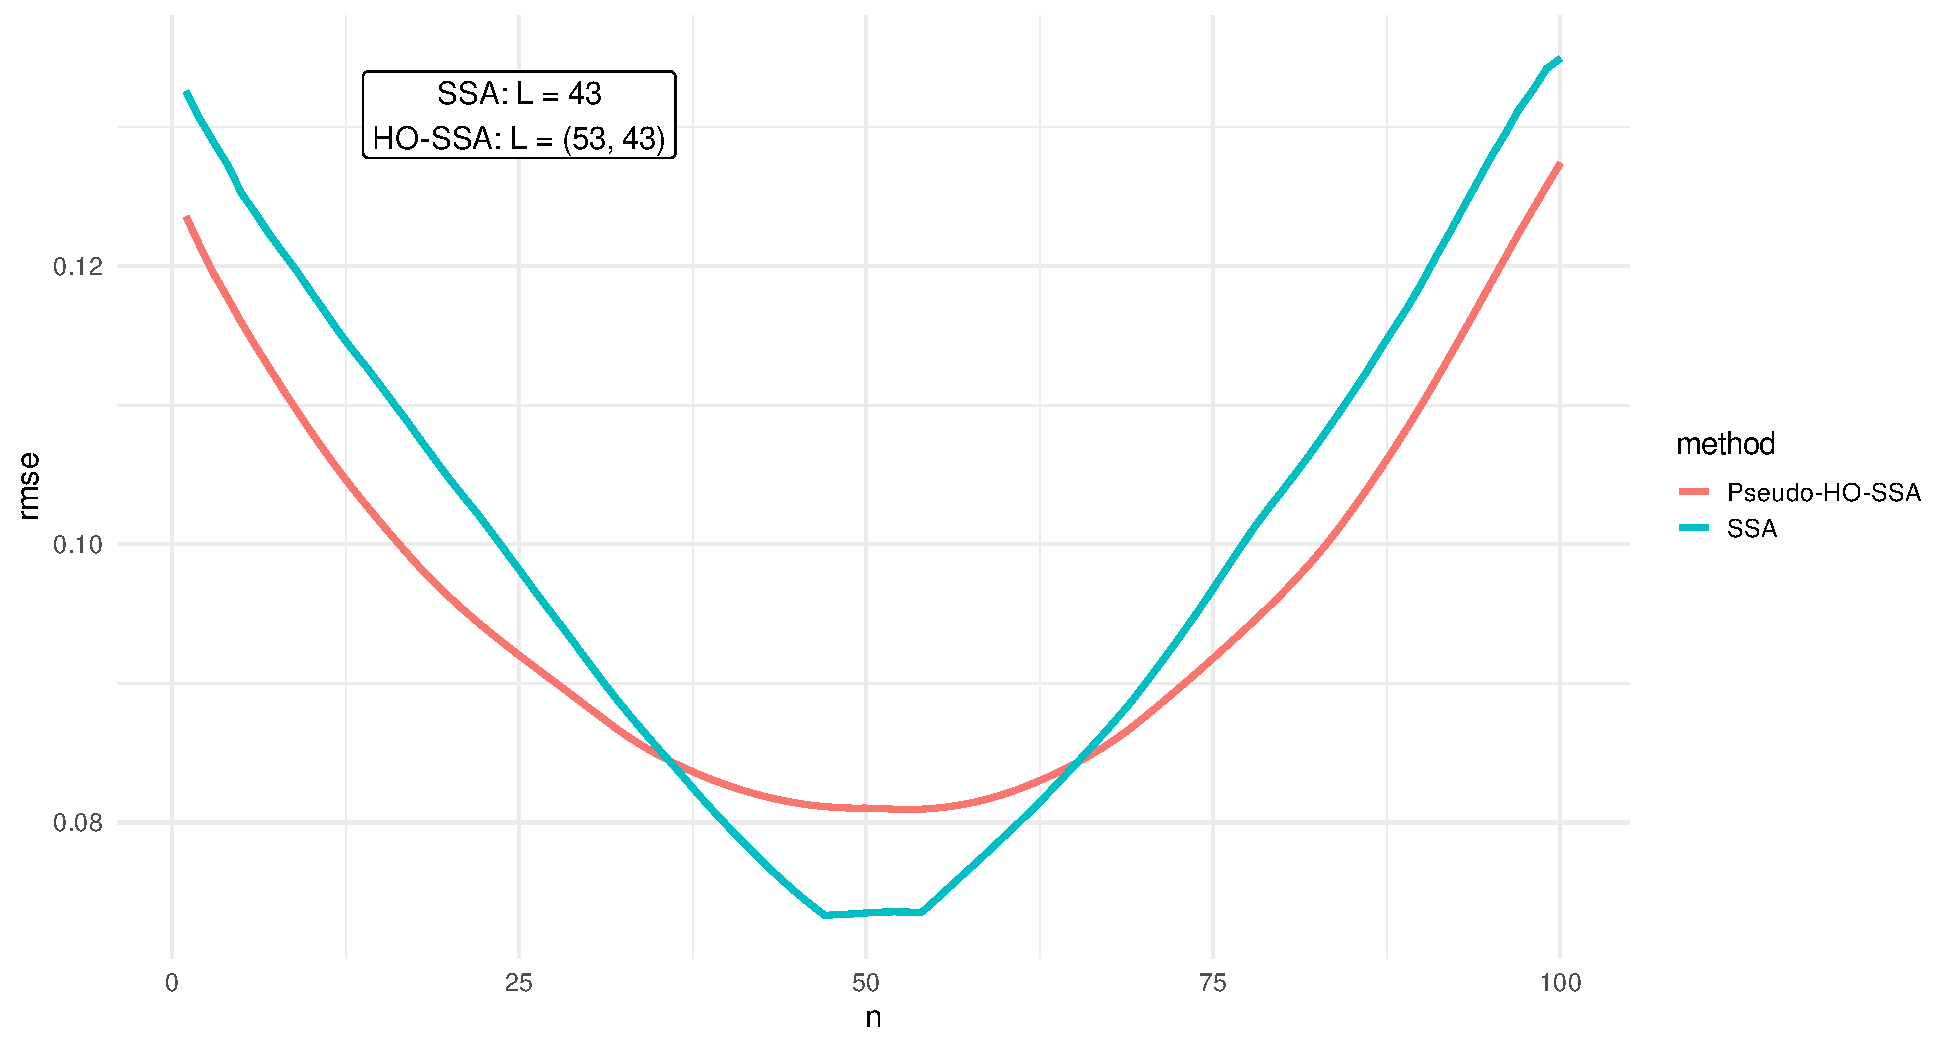
\includegraphics[width=\textwidth]{pw_const.pdf}
  \end{figure}
\end{frame}

\begin{frame}{Поточечное сравнение точности для сложного ряда}
  $x_{n} = e^{ \alpha_1 n } e^{2 \pi\mathrm{i} \omega_1 n} +
  e^{ \alpha_2 n } e^{ 2 \pi  \mathrm{i}\omega_2 n}$, $N = 100$
  \begin{figure}
    \centering
    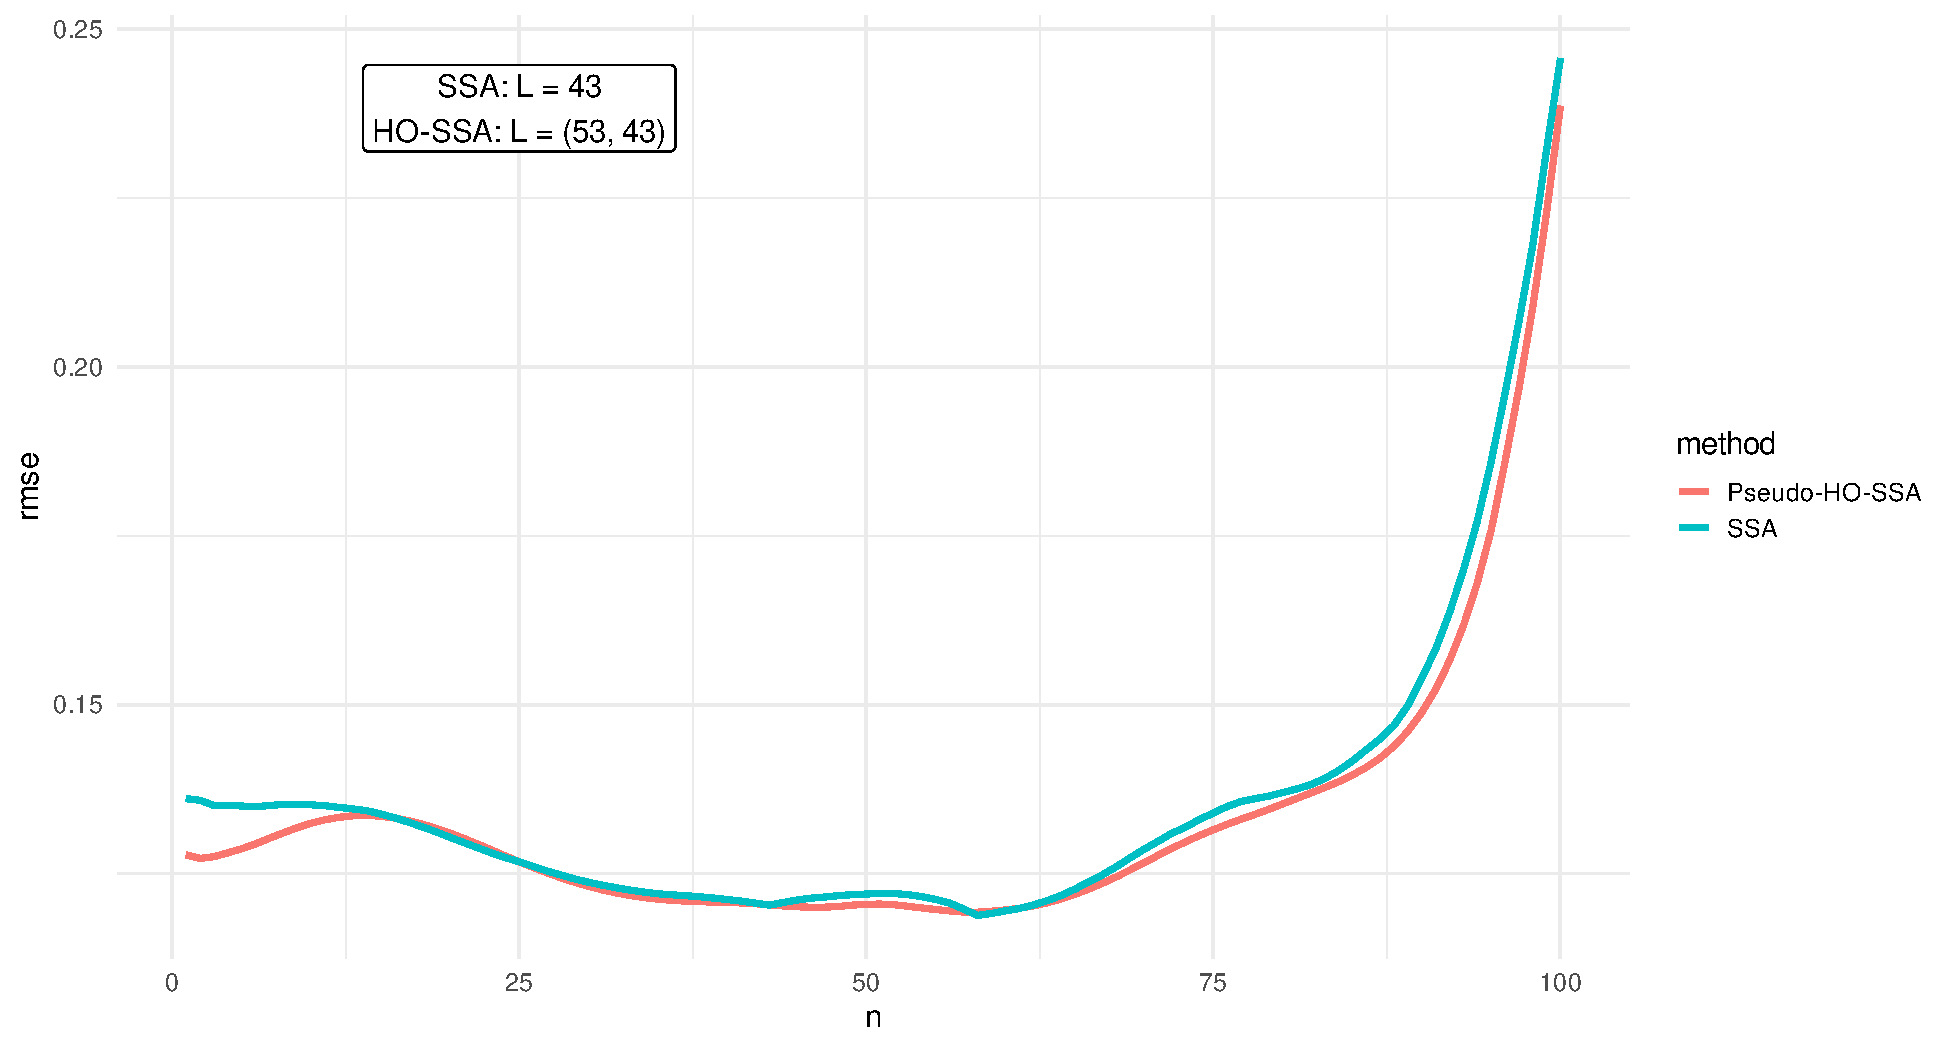
\includegraphics[width=\textwidth]{pw_complex_2_cos.pdf}
  \end{figure}
\end{frame}

\begin{frame}{Применение к космплексным многоканальным рядам}
  \[
    x_{n}^{(m)} = a_1^{(m)} e^{ \alpha_1 n }
    e^{2 \pi \mathrm{i} \omega_1 n} +
    a_2^{(m)} e^{ \alpha_2 n }
    e^{2 \pi \mathrm{i} \omega_2 n} + \zeta_n^{(m)},
  \]
  $N = 100$, $M=12$, $\zeta_n^{(m)}$ --- комплексный белый гауссовский шум,
  $\mathrm{D}\left(\zeta_n^{(m)}\right) = 0.6^2$, $\omega_1 = 0.2,\,
  \omega_2 = 0.22$, $\alpha_1=0.01$,
  $\alpha_2=0.02$.

  \medskip

  \begin{table}
    \centering
    \bluetext{Оптимальные по выбору длины окна значения RMSE}

    \begin{tabular}{c|c||c}
      \hline
      Задача & Выделение сигнала & Оценка параметров \\\hline
      Матричный метод & 0.101 ($L=73$) & 1.022e-04 ($L=53$) \\\hline
      Тензорный метод & \textbf{0.070} ($L=43$) & 1.017e-04 ($L=43$) \\\hline
    \end{tabular}
  \end{table}

  В задаче выделения сигнала тензорный метод значимо более точный.

  В задаче оценки параметров значимого различия точности методов не обнаружено.
\end{frame}

\section{Условия наибольшей точности T-MSSA}
\begin{frame}{Зависимость точности T-MSSA от числа каналов}
  \[
    x_n^{(m)} = (A_m (n - 1) + B_m) e^{-0.04 (n - 1)}\cos (2 \pi (n -
    1) / 5) + \xi_n^{(m)},
  \]
  $N = 25$, $r=4$, $r_3 = 2$, $A_m$, $B_m$ --- фиксированные
  константы, $\xi_n^{(m)}$ --- белый гауссовский шум

  \begin{table}[!ht]
    \centering
    \small
    \bluetext{Зависимость RMSE оценки сигнала от количества каналов и
    стандартного отклонения шума для методов MSSA (M) и T-MSSA (T)}
    \begin{tabular}{c|c|ccccccc}
      $\sigma$ & Метод & $M = 2$ & $M = 8$ & $M = 12$ & $M = 16$ & $M
      = 20$ & $M = 40$ \\ \hline
      \multirow{2}{1.3em}{0.2} & M & .11 & .10 &
      .10 & .10 & .09 & .09 \\
      & T & .11 & .08 & .08 & .07 & .07
      & .07 \\
      \hline
      \multirow{2}{1.3em}{0.4} & M & .23 & .20 &
      .19 & .19 & .19 & .19 \\
      & T & .23 & .18 & .16 & .15 & .15
      & .14 \\
      \hline
      \multirow{2}{1.3em}{0.6} & M & .34  & .30 &
      .29 & .29 & .28 & .28 \\
      & T & .34 & .26 & .22 & .24 & .23
      & .21 \\
      \hline
    \end{tabular}
  \end{table}

  При фиксированном $r_3$ преимущество T-MSSA увеличивается с
  увеличением количества каналов.
\end{frame}

\section{Оценка параметров с использованием Dstack}
\begin{frame}{Модификации Dstack}
  Возможная проблема при использовании ESPRIT: компоненты с близкими
  частотами могут смешиваться в одну при достаточно большом уровне шума.
  Решение: использование отображения Dstack [Morren~et~al.~(2003)].
  \medskip

  Пусть $\tX = (x_1,\, x_2,\, \ldots,\, x_N)$, $M = \lfloor N /
  D\rfloor$, тогда
  \[
    \operatorname{Dstack}_D(\tX) = \calD_D(\tX) =
    \left[
      \begin{NiceArray}{c|c|c|c}
        x_1 & x_2 & \ldots & x_{D} \\
        x_{D+1} & x_{D+2}  &\ldots &  x_{2D} \\
        x_{2D+1} & x_{2D+2} &\ldots & x_{3D} \\
        \vdots & \vdots & \ \cdots \  & \vdots \\
        x_{(M - 1)D+1} & x_{(M - 1)D+2}
        &\ldots & x_{MD} \\
        \CodeAfter
        \UnderBrace[shorten,yshift=1.5mm]{last-1}{last-1}{\tX_D^{(1)}}
        \UnderBrace[shorten,yshift=1.5mm]{last-2}{last-2}{\tX_D^{(2)}}
        \UnderBrace[shorten,yshift=1.5mm]{last-4}{last-4}{\tX_D^{(D)}}
      \end{NiceArray}
    \right]
  \]
  \vspace{0.3cm}

  \begin{table}
    \renewcommand{\arraystretch}{1.4}
    \begin{tabular}{r|l}
      Dstack-SSA & $\displaystyle\tX \mapsto \bfX=
      \calT_{\textrm{MSSA}}^{(L)} \left( \calD_D (\tX)\right)$\\\hline
      Dstack-T-SSA & $\displaystyle\tX \mapsto \calX=
      \calT_{\textrm{T-MSSA}}^{(L)} \left( \calD_D (\tX)\right)$
    \end{tabular}
  \end{table}

  Уменьшение разрешения: $\displaystyle\omega \mapsto \hat\omega=
  D \omega \implies$ необходимо $|\omega| \leqslant \frac{1}{2D}$
\end{frame}

\begin{frame}{Оценка параметров с использованием Dstack}
  \vspace*{-0.3cm}
  \[
    x_{n} = \cos(2 \pi \omega_1 n) +
    \cos(2 \pi \omega_2 n) + \xi_n
  \]
  $N = 990$, $D=10$, $\omega_1 = 0.02,\, \omega_2 = 0.0205$,
  $\xi_n$ --- белый гауссовский шум, $\mathrm{D}(\xi_n) = \sigma^2$\\ \smallskip

  RMSE посчитан по 100 реализациям

  \medskip

  \begin{table}
    \centering
    \bluetext{Оптимальные по выбору длины окна значения RMSE}

    \begin{tabular}{c|c||c}
      \hline
      & $\sigma = 0.2$ & $\sigma = 0.6$ \\\hline
      ESPRIT & 4.98e-05 ($L = 403$) & 0.101 ($L = 438$) \\\hline
      Dstack-ESPRIT & 5.30e-05 ($L = 60$) & 0.009 ($L=48$) \\\hline
      T-Dstack-ESPRIT & 5.40e-05 ($L = 41$) & \textbf{0.003} ($L = 46$) \\\hline
    \end{tabular}
  \end{table}

  Полученные результаты подтверждают выводы [Papy et al. (2008)] о
  преимуществе T-ESPRIT с применением Dstack при близких частотах и
  высоком уровне шума.
\end{frame}

% \begin{frame}{Разделимость и ранги рядов в терминах SSA}
%   \begin{itemize}
%     \item \bluetext{Выделение сигнала:} нахождение ранга
% ряда\\ \vspace{0.1cm}
%       {\small
%         Пусть $\tS$ --- сигнал, $\bfS_L$ --- его траекторная матрица с
%       длиной окна $L$.}
%       \begin{definition}[Ранг сигнала в терминах SSA]
%         $\tS$ имеет ранг $R$, если $R \leqslant N/2$ и $\forall L$:
%         $R\leqslant \min(L, N-L+1)$\\
%         $\operatorname{rank}(\bfS_L)=R$
%       \end{definition}
%     \item \bluetext{Разделение составляющих сигнала} пусть $\tS =
%       \tS_1 + \tS_2$,\\
%       {\small $\bfS$, $\bfS_1$, $\bfS_2$ --- траекторные матрицы этих
%       сигналов с длиной окна $L$}
%       \begin{definition}[Разделимость в терминах SSA]
%         Сигналы $\tS_1$ и $\tS_2$ $L$-разделимы, если существуют
%         такие $\gI_1, \gI_2$, что
%         \[
%           \bfS = \sideset{}{_{j=1}^R}\sum\nolimits \sqrt{\lambda_j}
%           U_j V_j^{\Tp} =
%           \overbrace{\sideset{}{_{j\in \gI_1}}\sum\nolimits
%           \sqrt{\lambda_j} U_j V_j^{\rmT}}^{\bfS_1} +
%           \overbrace{\sideset{}{_{j\in \gI_2}}\sum\nolimits
%           \sqrt{\lambda_j} U_j V_j^{\rmT}}^{\bfS_2}
%         \]
%       \end{definition}
%   \end{itemize}
% \end{frame}
% \begin{frame}{HO-SSA: $n$-ранги траекторного тензора}
%   \begin{theorem}[О связи рангов рядов в SSA и HO-SSA]
%     Пусть сигнал $\tS$ имеет SSA-ранг $R$.\\
%     Тогда для любых $L$ и $K$ таких, что
%     \[
%       R \leqslant \min(L, K, N-L-K+2),
%     \]
%     $\rank_1(\calS)=\rank_2(\calS)=\rank_3(\calS)=R$,
%     где $\calS$ --- траекторный тензор $\tS$, построенный по длинам
%     окна $L$, $K$.
%   \end{theorem}
%   \vspace{0.4cm}

%   Теорема позволяет использовать известные результаты о рангах
%   сигналов из теории \textup{SSA} для
%   аппроксимации траекторного тензора на шагах разложения и
%   группировки в методе \textup{HO-SSA}.
% \end{frame}
% \begin{frame}{HO-SSA: разделимость}
%   Пусть $\tS = \tS_1 + \tS_2$,\\
%   $\calS$, $\calS_1$, $\calS_2$ --- траекторные тензоры этих сигналов
%   с длинами окна $L$ и $K$
%   \begin{theorem}[О связи разделимости в SSA и HO-SSA]
%     HOSVD тензора $\mathcal{S}$ можно представить в виде
%     суммы HOSVD тензоров $\calS_1$ и $\calS_2$ тогда и только тогда,
%     когда сигналы $\tS_1$ и $\tS_2$ $L$- и $K$-разделимы в терминах SSA.
%   \end{theorem}
%   \vspace{0.4cm}
%   Теорема позволяет выделить класс сигналов, которые можно
%   разделить методом HO-SSA, а также даёт рекомендации к выбору
%   параметров $L$ и $K$.
% \end{frame}
% \begin{frame}{HOSVD-MSSA: $n$-ранги траекторного тензора}
%   \begin{theorem}[О $n$-рангах траекторного тензора многоканального ряда]
%     Пусть $\tS = \left(\tS^{(1)} : \ldots : \tS^{(Q)}\right)$, тогда
%     справедливы следующие утверждения.
%     \begin{enumerate}
%       \item $\tS$ имеет MSSA-ранг $R$
%         тогда и только тогда, когда для траекторного тензора $\calS$,
%         построенного по любой длине окна $L<N$ такой, что
%         $R \leqslant\min(L, N - L + 1)$ выполняется
%         \[\operatorname{rank}_1(\calS) =
% \operatorname{rank}_2(\calS) = R.\]
%       \item $\operatorname{rank}_3(\calS)$ равен рангу матрицы,
%         в строках которой содержатся каналы $\tS^{(q)}$ сигнала.
%     \end{enumerate}
%   \end{theorem}
%   \vspace{0.2cm}
%   Теорема позволяет использовать известные результаты о MSSA-рангах
%   сигналов из теории для аппроксимации траекторного тензора по первым двум
%   направлениям, а также даёт рекомендации к
%   выбору ранга аппроксимации по третьему направлению на шагах
%   разложения и группировки в методе HOSVD-MSSA.
% \end{frame}

% \begin{frame}{HOSVD-MSSA: разделимость}
%   Пусть $\tS = \tS_1 + \tS_2$, \\
%   $\calS$, $\calS_1$, $\calS_2$ --- траекторные тензоры этих
% сигналов с длиной
%   окна $L$\\ \vspace{0.2cm}
%   $\Lambda^{(I)}(\tS) = \operatorname{span}\left\{\left(s_i^{(q)},
%   s_{i+1}^{(q)}, \ldots, s_{i + I - 1}^{(q)}\right)\right\}$
%   \begin{theorem}[О разделимости методом HOSVD-MSSA]
%     HOSVD тензора $\calS$ можно представить в виде суммы
%     HOSVD тензоров $\calS_1$ и
%     $\calS_2$ тогда и только тогда, когда
%     $\Lambda^{(L)}(\tS_1) \perp \Lambda^{(L)}(\tS_2)$ и
%     $\Lambda^{(K)}(\tS_1)\perp\Lambda^{(K)}(\tS_2)$
%   \end{theorem}
%   \vspace{0.2cm}
%   Теорема позволяет выделить класс сигналов, которые можно
%   разделить методом HOSVD-MSSA,
%   а также даёт рекомендации к выбору параметра $L$.
% \end{frame}

\section{Полученные результаты. Сравнение методов}
\begin{frame}{Сравнение точности одноканальных методов}
  \begin{itemize}
    \item T-SSA с использованием HOSVD существенно менее
      точный, чем SSA во всех рассмотренных случаях комплексных рядов\smallskip
    \item T-SSA с использованием Pseudo-HOSVD более
      точный, чем SSA в задачах выделения сигнала и оценки параметров
      в рассмотренных случаях\smallskip
    \item Значимого различия между методами в задаче оценки
      параметров не обнаружено.
    \item Подтверждены результаты статьи [Papy et al. (2008)] о том,
      что при достаточно близких частотах и высоком уровне шума
      ESPRIT перестаёт идентифицировать все параметры сигнала;\\
      T-ESPRIT с использованием Dstack даёт возможность в этих
      условиях оценивать параметры с более высокой точностью.\smallskip
    \item Трудоёмкость тензорных методов имеет тот же порядок, что и
      матричных, но с большей константой.
  \end{itemize}
\end{frame}

\begin{frame}{Сравнение точности многоканальных методов}
  \bluetext{Было известно:} [Papy et al. (2005), Хромов (2024)]
  \begin{itemize}
    \item В условиях одинакового уровня шума во всех каналах точность
      тензорных методов (T-MSSA, T-M-ESPRIT) выше, чем матричных (MSSA,
      M-ESPRIT)\smallskip
    \item Условия слабой T-MSSA-разделимости более строгие, чем
      условия MSSA-разделимости;\\
      На практике, ошибка, возникающая при наличии
      MSSA-разделимости и отсутствии T-MSSA-разделимости, довольно мала
  \end{itemize}\medskip

  \bluetext{Новый результат:}
  \begin{itemize}
    \item Если 3-ранг ряда совпадает с количеством каналов, то
      различие ошибок методов невелико\smallskip
    \item С увеличением количества каналов разница в точности
      растёт в пользу тензорных методов\smallskip
    \item Трудоёмкость тензорных методов имеет тот же порядок, что и
      матричных, но с большей константой.
  \end{itemize}
\end{frame}

\section{Заключение}
\begin{frame}{Дальнейшая работа}
  Наиболее перспективно --- изучение свойств T-SSA с использованием
  Pseudo-HOSVD и свойств T-MSSA\bigskip
  \begin{itemize}
    \item Сравнение Pseudo-HO-SSA в задаче разделения компонент,
      вложенный вариант Pseudo-HO-SSA $\rightarrow$ HO-SSA\medskip
    \item Нахождение рекомендаций к выбору параметров длины окна в
      методе Pseudo-HO-SSA\medskip
    \item Дальнейшее изучение поведения сингулярных чисел сигналов\medskip
    \item Сравнение методов по уровню шума, при котором
      происходит смешивание компонент сигнала с шумом\medskip
    \item Определение разделимости по вкладам и сильной
      разделимости на языке тензорных методов\medskip
    \item Исследование ошибок первого порядка при
      аппроксимации тензора разложением\medskip
  \end{itemize}
\end{frame}
\end{document}